%%%%%%%%%%%%%%%%%%%%%%%%%%%%%%%%%%%%%%%%%%%%%%%%%%%%%%%%%%%%%%%%%%%%%%%%%%%%%%%%

\documentclass[letterpaper, 10 pt, conference]{ieeeconf}  % Comment this line out
                                                          % if you need a4paper
%\documentclass[a4paper, 10pt, conference]{ieeeconf}      % Use this line for a4
                                                          % paper

\IEEEoverridecommandlockouts                              % This command is only
                                                          % needed if you want to
                                                          % use the \thanks command
\overrideIEEEmargins
% See the \addtolength command later in the file to balance the column lengths
% on the last page of the document

\usepackage[utf8]{inputenc}
\usepackage[T1]{fontenc}
\usepackage{graphicx}
\usepackage{cite}
\usepackage{amsmath,amssymb,amsfonts}
\usepackage{algorithmic}
\usepackage{graphicx}
\usepackage{adjustbox}
\usepackage{textcomp}
\usepackage{xcolor}
\usepackage{algorithm2e}
\usepackage{threeparttable,tabularx,booktabs,makecell}
\usepackage{stfloats}
\usepackage{floatrow}
\usepackage{float}
\floatstyle{plaintop}
\restylefloat{table}
\usepackage{array}
\usepackage{booktabs}

% The following packages can be found on http:\\www.ctan.org
%\usepackage{graphics} % for pdf, bitmapped graphics files
%\usepackage{epsfig} % for postscript graphics files
%\usepackage{mathptmx} % assumes new font selection scheme installed
%\usepackage{mathptmx} % assumes new font selection scheme installed
%\usepackage{amsmath} % assumes amsmath package installed
%\usepackage{amssymb}  % assumes amsmath package installed

\title{\LARGE \bf
Evaluating PPG Signal Quality Across Skin Tones using Signal Metrics
}

%\author{ \parbox{3 in}{\centering Huibert Kwakernaak*
%         \thanks{*Use the $\backslash$thanks command to put information here}\\
%         Faculty of Electrical Engineering, Mathematics and Computer Science\\
%         University of Twente\\
%         7500 AE Enschede, The Netherlands\\
%         {\tt\small h.kwakernaak@autsubmit.com}}
%         \hspace*{ 0.5 in}
%         \parbox{3 in}{ \centering Pradeep Misra**
%         \thanks{**The footnote marks may be inserted manually}\\
%        Department of Electrical Engineering \\
%         Wright State University\\
%         Dayton, OH 45435, USA\\
%         {\tt\small pmisra@cs.wright.edu}}
%}

\usepackage{authblk}

\author[1]{Jessica Li}
\author[1]{Nate Sowder}
\affil[1]{Department of Computer Science, Northwestern University, Evanston, IL}

% \author{Jessica Li$^{1}$ and Nate Sowder$^{1}$ % <-this % stops a space 
% \thanks{*This work was not supported by any organization}% <-this % stops a space
% \thanks{$^{1}$H. Kwakernaak is with Faculty of Electrical Engineering, Mathematics and Computer Science,
%         University of Twente, 7500 AE Enschede, The Netherlands
%         {\tt\small h.kwakernaak at papercept.net}}%
% \thanks{$^{2}$P. Misra is with the Department of Electrical Engineering, Wright State University,
%         Dayton, OH 45435, USA
%         {\tt\small p.misra at ieee.org}}%
% }


\begin{document}



\maketitle
\thispagestyle{empty}
\pagestyle{empty}


%%%%%%%%%%%%%%%%%%%%%%%%%%%%%%%%%%%%%%%%%%%%%%%%%%%%%%%%%%%%%%%%%%%%%%%%%%%%%%%%
\begin{abstract}
In this study, we investigate the relationship between skin pigmentation and photoplethysmography (PPG) signal quality by analyzing different wavelength combinations in controlled laboratory conditions. Identifying optimal wavelengths based on skin pigmentation can significantly enhance the accuracy of PPG measurements on wearable devices, such as smartwatches. By calibrating devices to account for the user's skin tone, measurement errors may be reduced, particularly addressing the disparity in measurement quality often experienced between lighter and darker skin tones. Given that most wearable devices currently perform better on individuals with lighter skin, as highlighted by prior research \cite{bent_investigating_2020}, we hope to expand upon past literature in this area to increase accessibility and reduce bias in healthcare outcomes.
\end{abstract}


%%%%%%%%%%%%%%%%%%%%%%%%%%%%%%%%%%%%%%%%%%%%%%%%%%%%%%%%%%%%%%%%%%%%%%%%%%%%%%%%
\section{INTRODUCTION}

Photoplethysmography (PPG) has gained popularity as a non-invasive method of measuring heart rate in patients. Furthermore, PPG has recently seen novel applications in measuring patient blood pressure \cite{elgendi_photoplethysmography_2024} in a similar non-invasive manner, without the need for mechanical cuffs. However, PPG can be prone to noisy signals, because the light refractions it detects can vary with the environment and the individual \cite{castaneda_review_2018}. In fact, recent literature suggests that skin pigmentation can affect the reading quality of PPG \cite{al-halawani_review_2023}, and that the light wavelength used by the PPG device can also affect the reading quality \cite{fallow_influence_2013}. However, studies that have explored the effect of skin pigmentation on the quality of PPG used dated and subjective measurements of skin tone. These skin tone classifications are prone to errors due to observer bias, lighting conditions, and bias in self-reporting \cite{vasudevan_melanometry_2024}. This poses a problem for the measurement quality of PPG sensing for people of different skin tones. We focus on evaluating the most effective wavelength or combination of wavelengths for people of different skin tones and providing more information on the effect of skin pigmentation on PPG reading. To improve on previous research, we propose using measuring tools such as colorimeters to ensure a more robust categorization of skin pigmentation. Specifically, we used a colorimeter that expresses color in the CIELAB color space defined by the International Commission on Illumination. This measurement tool and metric provides a more reliable measurement of skin tone due to the CIELAB color space being designed to represent human color perception and providing an objective quantification of skin pigmentation that is independent of observer bias \cite{ly_research_2020}. We also expand on the current literature by increasing the types of wavelengths that have been tested, including intermediate visible and infrared wavelengths. 

Our study was performed by recruiting participants of a variety of skin tones and measuring their skin pigmentation in a fluorescent-lit room at room temperature to ensure consistent lighting and temperature conditions. We used ExtHub, a wearable device that includes red, orange, green, and infrared wavelengths to collect PPG on the participants. The device was worn on the participant’s right wrist, and data was collected for each wavelength while the participant is sitting at rest. We preprocessed the raw PPG data and utilized statistical evaluation techniques to assess the quality of the PPG signal.
% and employing machine learning models such as convolutional neural networks (CNNs) and long short-term memory networks (LSTMs) trained on an open source dataset with classified good and bad quality PPG signal reads. 
We used the signal quality metrics to split PPG readings into "good" and "bad" quality readings. We analyzed the frequency of good and bad quality PPG signals across the varied wavelengths for each categorized skin tone in order to determine whether there existed a correlation between skin tone and PPG reading, and what role wavelength played upon this correlation (if any).

\section{Related Works}
Current PPG sensors utilize one or more light-emitting diodes (LEDs) to capture the intensity of non-absorbed light reflected from the tissue \cite{castaneda_review_2018}. The most prevalent LED colors are green, red, and yellow, with red being the longest wavelength and green being the shortest wavelength of the three. Studies have determined that light with longer wavelengths will penetrate deeper into the tissue compared to light with shorter wavelengths \cite{fallow_influence_2013}\cite{setchfield_effect_2024}. However, the range of electromagnetic wavelengths have historically been quite limited. Studies which include PPG sensor light wavelength variability have only tested within the range of visible light \cite{al-halawani_review_2023}\cite{fallow_influence_2013}. We seek to expand the current literature by testing on infrared light in addition to visible light, and use combinations of wavelengths as well.

Additionally, researchers have found that darker skin tones were correlated with lower accuracy in biological markers derived from PPG signals \cite{al-halawani_review_2023}\cite{bent_investigating_2020}. To account for this, previous studies have categorized skin pigmentation on scales such as the Fitzpatrick skin type scale (FST) and measured absorption and scattering coefficients with varying wavelengths \cite{setchfield_effect_2024}. Specifically to PPG signals, previous research has also examined the effectiveness of using multiple wavelengths to collect PPG data \cite{ray_review_2023}, however many studies rely on constricting skin pigmentation categorization methods such as FST, which constrains classification to a smaller range of skin tones \cite{okoji_equity_2021}. While such efforts at aligning PPG quality and skin classification are well-intentioned, historical skin classification systems such as the FST are prone to subjectivity and bias, often struggling to classify based on naked-eye observation and self-reporting alone \cite{fitzpatrick_validity_1988}. Our work aims to combine the spirit of previous studies insofar as testing the effectiveness of PPG reading on different skin pigmentations with colorimetry as supported through the CIELAB color space. 

% A similar study conducted by Fallow et al. tested different wavelengths and skin types for measuring PPG, but their research was targeted towards finding suitable wavelengths for signal detection during exercise versus at rest \cite{fallow_influence_2013}. We will focus more on testing the efficacy of single wavelengths for different categories of skin tone at resting state for participants. Our focus targets the disparity in accuracy of PPG measurement for patients with darker skin tones compared to patients with lighter skin tones.

% Machine learning methods have been utilized in the realm of PPG signal processing, with more research focusing on using models to analyze blood pressure, sleep quality, mental health, etc. from PPG signals \cite{nie_review_2024}\cite{gonzalez_benchmark_2023}. Assessment of PPG signal quality has been conducted before, however researchers focused on PPG signals with presence of episodic heart arrhythmia \cite{pereira_deep_2019}, and provided a quality assessment model utilizing heart rate and heart rate variability parameters \cite{naeini_deep_2023}. Therefore, we propose to provide a benchmark assessment of methods in quantifying PPG signal quality.
% , CNNs, LSTMs, and support vector machines (SVMs).

\section{Methods}
Our study aims to investigate the effect of PPG signal quality and accuracy across different skin tones. We recruited participants with diverse skin tones, measured their pigmentation using CIELAB values, and collected PPG signals under controlled conditions using multiple wavelengths and combinations. Signal quality was evaluated using statistical metrics, including signal-to-noise ratio (SNR), entropy, and a heart rate deviation score, to determine the impact of skin tone on PPG accuracy.

\subsection{Device}
We use ExtHub, a wearable bluetooth device that can be strapped on to the forearms or upper arms. The device features a three axis accelerometer, five light emitting diodes (LEDs) as photoplethysmography (PPG) sensors, and an electrocardiogram (ECG) sensor. For this study, we only use the PPG sensors, which can be customized by frequency, integration cycles, sequence repeats, and the gains of two transimpedance amplifier channels. The device has the option to change the light wavelengths used during the measurement period. The wavelengths include, green, orange, red, and infrared, and the electrical current for each wavelength can be changed from the range of 0 to 250 milliamperes (mAs). For our study, we strap on the ExtHub sensors to the anterior forearm, with the placement of the sensor approximately in the middle of the wrist and elbow. We also use a constant sampling frequency of 50 hertz (Hz), 1 integration cycle, 16 sequence repeats, and gains of 20 thousand Ohms for both channels.

\subsection{Participants and Data Collection Procedure}
Our study was conducted with 15 adult participants. We aim to recruit participants of different skin tones to provide a diverse cohort because the general goal of the study is to determine which wavelengths provide quality PPG signals for people of various skin tones. We first prompted participants to self-select the closest option to their anterior forearm’s skin tone based on an eleven color palette. Then to obtain a quantitative measurement of skin tone, we photographed the participants’ anterior forearms and used the Trigit web application \cite{tjandra_trigit_2023} to determine the lightness (L*), red/green (a*), and yellow/blue (b*) values of the CIELAB color space. To minimize random error, we performed three repeated measurements of skin tone with three images of the participants’ anterior forearms and averaged the three values. We collected data in a well lit and windowless room to ensure lighting changes did not impact the CIELAB calculation and PPG signal collection. During the data collection period, each participant was instructed to stay seated and to refrain from moving the arm that wore the ExtHub device. We recorded PPG signals using red, green, orange, and infrared wavelengths separately for 30 seconds each with a fixed electrical current of 100 mA. Additionally, we recorded combinations of wavelengths, including only visible light (red, green, orange), green and infrared, and green and red wavelengths.

\subsection{Skin Pigmentation Interpretation}
\begin{figure}
    \centering
    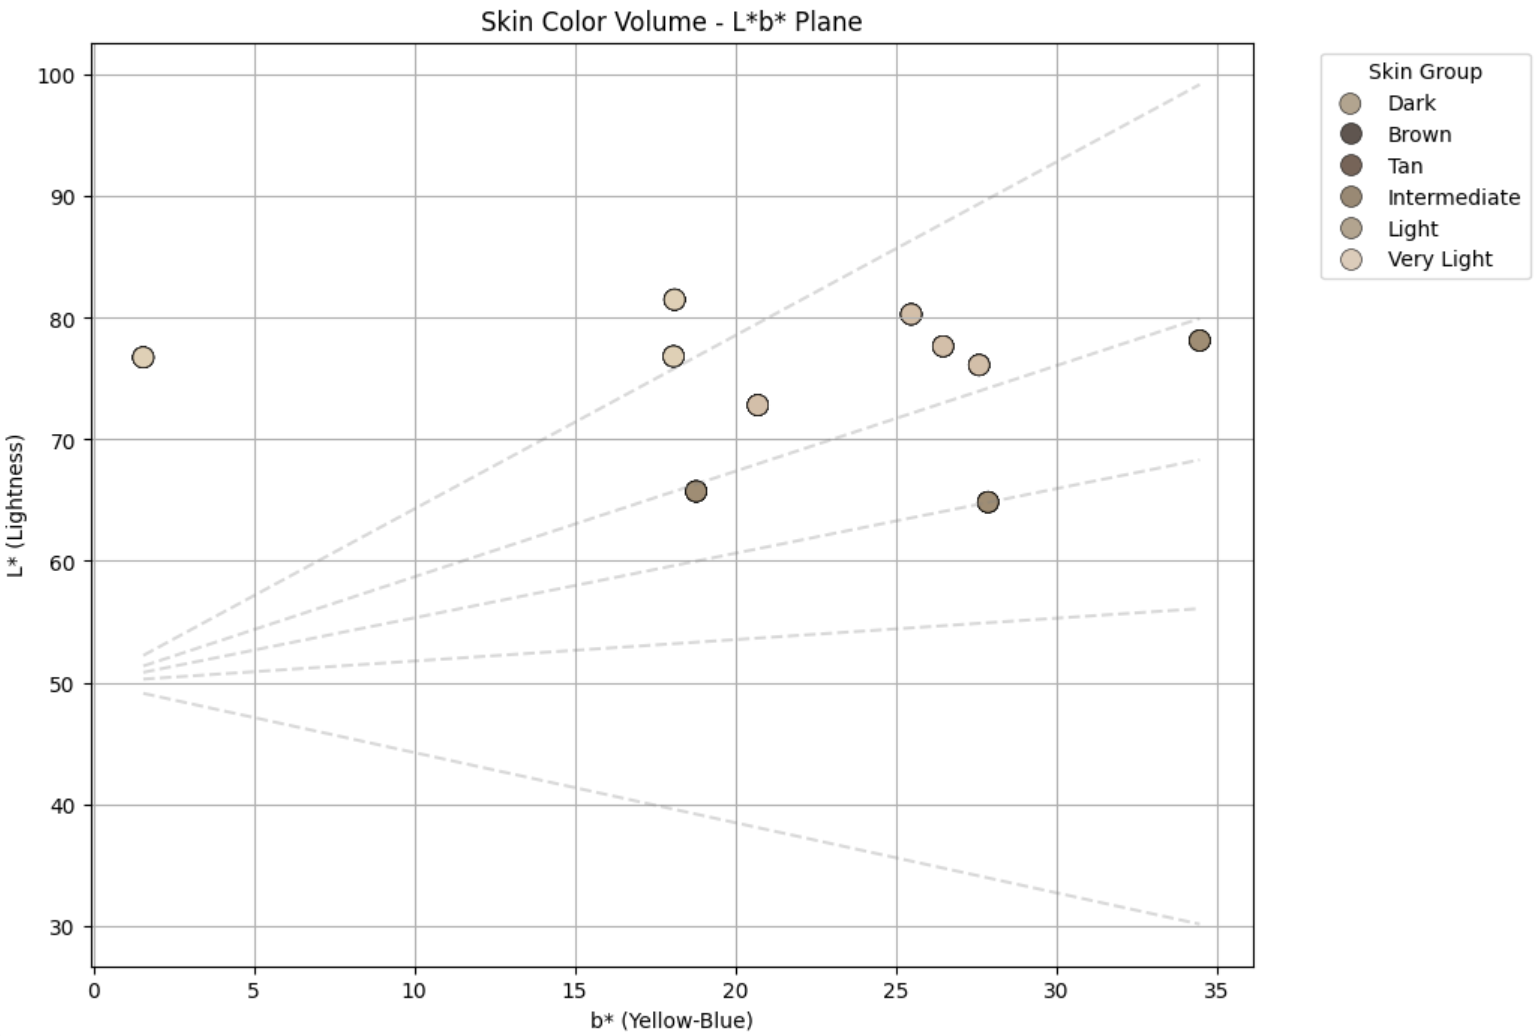
\includegraphics[width=\linewidth]{images/skincolor.png}
    \caption{X-axis: b* (Higher b* corresponds to greater yellow component). Y-axis: L* (Higher L* corresponds to greater perceptual lightness. Dashed lines are separators for skin pigmentation groups.}
    \label{fig:skincolor}
\end{figure}

To visualize the distribution of skin pigmentation for our participants and group similar skin tones together, we used the Individual Topology Angle (ITA), which uses L* and b* values to correspond skin color to one of six groups \cite{ly_research_2020}. \ref{fig:skincolor} shows the spread of associated skin tone for the participants.


\subsection{Preprocessing}
In order to retain the features of good and bad quality PPG signals, we applied minimal preprocessing steps to our raw data. The raw signals for green, red, and orange wavelengths are segmented into 20 second non-overlapping intervals. For the green and red, green and infrared, and visible light combinations, we align the separate wavelengths onto the same time axis with cubic interpolation, normalize the magnitude of the signals using the alternating and direct currents, and taking the average of the respective signals to achieve the respective combination. 

\subsection{Signal Quality Assessment}
% We train and evaluate a neural network along with statistical signal quality metrics to compare the types of wavelengths to signal measurement quality for different skin tones. 
The signal metrics we evaluated are Signal Noise Ratio (SNR), Kurtosis, Shannon Entropy (SE), and a heart rate variability score. We selected these metrics because PPG signals are primarily used to measure heart rate. To accurately measure heart rate, a high-quality signal should exhibit consistent pulse waves with a distinct pulse peak.

% We also tested a hybrid neural network consisting of convolutional and long short-term memory layers. 

We calculate SNR with respect to the signal power and noise power. To determine a noisy signal, we apply a Butterworth band pass filter with lower and upper thresholds of 0.7 and 3.5 on the raw signal and calculate the difference between the filtered signal and the raw signal. Kurtosis is calculated using Pearson's definition. The probability distribution function needed for SE is calculated by creating a histogram of 10 bins to find the probability distribution of the signal, then entropy is calculated with the probability distribution function. The heart rate variability score is a score that determines how much the estimated heart rate for one wavelength type varies compared to the average heart rate for the participant, with 0 signifying an estimated heart rate further away from the average and 1 signifying an estimated heart rate with the same value as the average. To determine the estimated heart rate, we use the HeartPy library and extract the beats per minute from the processed signal \cite{gent_analysing_2018}. Average heart rate is recorded by averaging the estimated heart rates across all wavelengths for each participant. We calculate a penalty score that represents how much each estimated heart rate deviates from the average heart rate.
We observe some flatlining PPG signals, notably in the infrared and red wavelengths. The metrics for these signals are null values.

Signal quality is determined as a binary indicator, with 0 indicating a bad signal and 1 indicating a good signal. Given the previously calculated metrics, we assign a threshold to each metric: the signal-to-noise ratio must be greater than 0, which indicates the signal is stronger than the relative noise; the kurtosis is be less than or equal to 3.5, which was determined as a suitable threshold in previous literature \cite{selvaraj_statistical_2011}; the entropy must be greater than or equal to 0.8, also following previous literature \cite{selvaraj_statistical_2011}; and the penalty score must be greater than or equal to 0.67, which corresponds to being within one standard deviation of the mean average heart rate. To classify a signal as good, at least three out of the four conditions must be met, otherwise the signal is classified as bad. For null value metrics, we automatically classify the signal as a bad signal.

\section{Results}
Figures 2 and 3 illustrate the distribution of skin pigmentation across various PPG wavelengths, employing both CIELab-measured values and self-reported skin pigmentation scales. Each figure presents these distributions separately,  split on the quality indicator of the PPG signal.

Table I presents a  summary of the aggregate mean scores and their associated standard deviations for each evaluated wavelength across our chosen PPG signal quality metrics. 

Table II details the Spearman correlation coefficients and p-values between skin pigmentation measurements and our PPG signal quality metrics. The table is split by skin pigmentation measurement technique. 
\begin{table*}[!t]
\centering
\begin{tabular}{@{}lcccccccc@{}}
\toprule
& \multicolumn{2}{c}{SNR} & \multicolumn{2}{c}{Kurtosis} & \multicolumn{2}{c}{Shannon Entropy} & \multicolumn{2}{c}{Heart Rate Score} \\ \midrule
Wavelength Type   & M & SD & M & SD & M & SD & M & SD \\ \midrule
Green             & -9$\times10^{-6}$   & 7.8$\times10^{-5}$  & 2.326  & 0.717  & 2.099  & 0.115  & 0.757  & 0.114  \\
Orange            & -4$\times10^{-6}$   & 1.24$\times10^{-4}$ & 2.812  & 1.139  & 2.035  & 0.159  & 0.717  & 0.203  \\
Red               & -5.6$\times10^{-5}$ & 1.94$\times10^{-4}$ & 2.673  & 1.269  & 2.021  & 0.188  & 0.715  & 0.227  \\
Infrared          & -1.2$\times10^{-5}$ & 3.4$\times10^{-5}$  & 2.629  & 0.336  & 1.974  & 0.027  & 0.797  & 0.145  \\
Green and Red     & -2.7$\times10^{-5}$ & 3.2$\times10^{-5}$  & 2.308  & 0.696  & 2.059  & 0.093  & 0.642  & 0.212  \\
Green and Infrared & -1.5$\times10^{-5}$ & 4.0$\times10^{-5}$  & 3.882  & 3      & 1.786  & 0.584  & 0.777  & 0.226  \\
Visible Light     & 1.36$\times10^{-4}$ & 3.93$\times10^{-4}$ & 2.805  & 0.632  & 2.075  & 0.095  & 0.737  & 0.184  \\ \bottomrule
\end{tabular}
\caption{Mean (M) and standard deviation (SD) values of PPG signal quality metrics for different wavelength types.}
\label{fig:4}
\end{table*}


\begin{table*}[t]
    \centering
    \begin{tabular}{p{4cm} p{3cm} r r}
    \toprule
    Skin Tone Metric & Quality Metric &  Spearman Correlation &  p-value \\
    \midrule
    Individual Topology Angle & SNR & 0.04653 & 0.72638 \\
     & Kurtosis & 0.04383 & 0.74171 \\
     & Shannon Entropy & -0.07458 & 0.57452 \\
     & Penalty Score & -0.07632 & 0.56564 \\
    Self-Reported Skin Tone & SNR & 0.00173 & 0.98960 \\
     & Kurtosis & -0.05074 & 0.70270 \\
     & Shannon Entropy & 0.02920 & 0.82620 \\
     & Penalty Score & -0.09799 & 0.46031 \\
    \bottomrule
    \end{tabular}
    
    \caption{Spearman correlation and p-value between skin tone and PPG signal quality metrics.}
    \label{fig:5}
\end{table*}



\begin{figure}
    \centering
    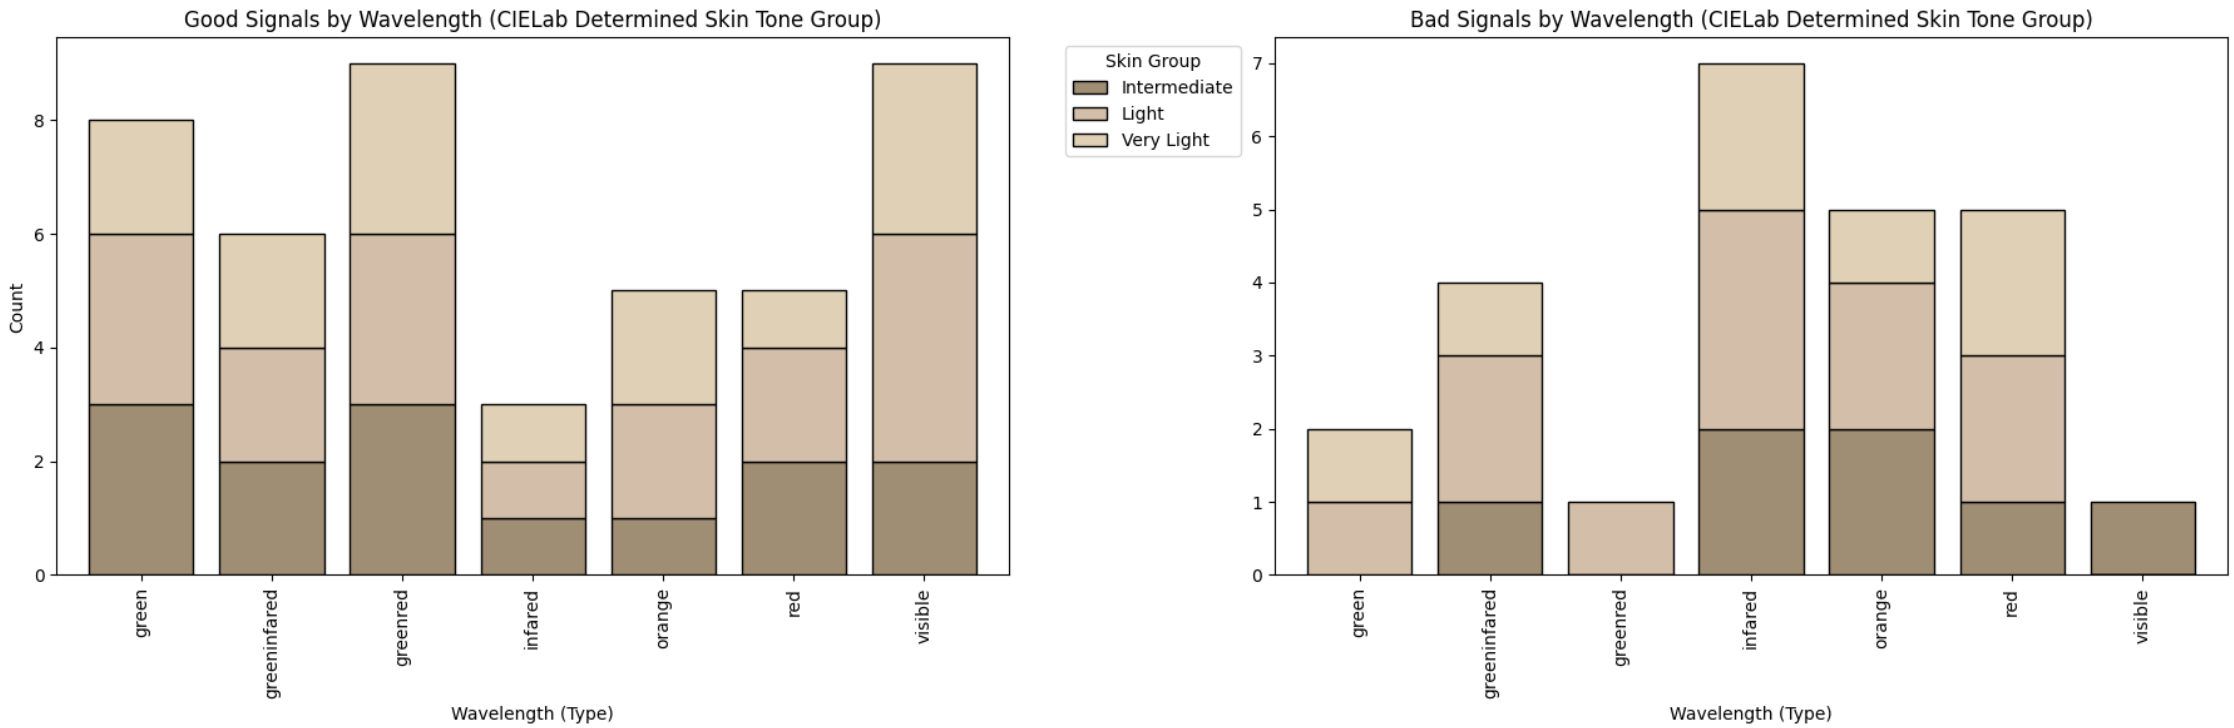
\includegraphics[width=\linewidth]{images/cielab_hist.png}
    \caption{Signal Quality by Wavelength, stratified by skin tone in the CIELab color space.}
    \label{fig:cielab_hist}
\end{figure}
\begin{figure}
    \centering
    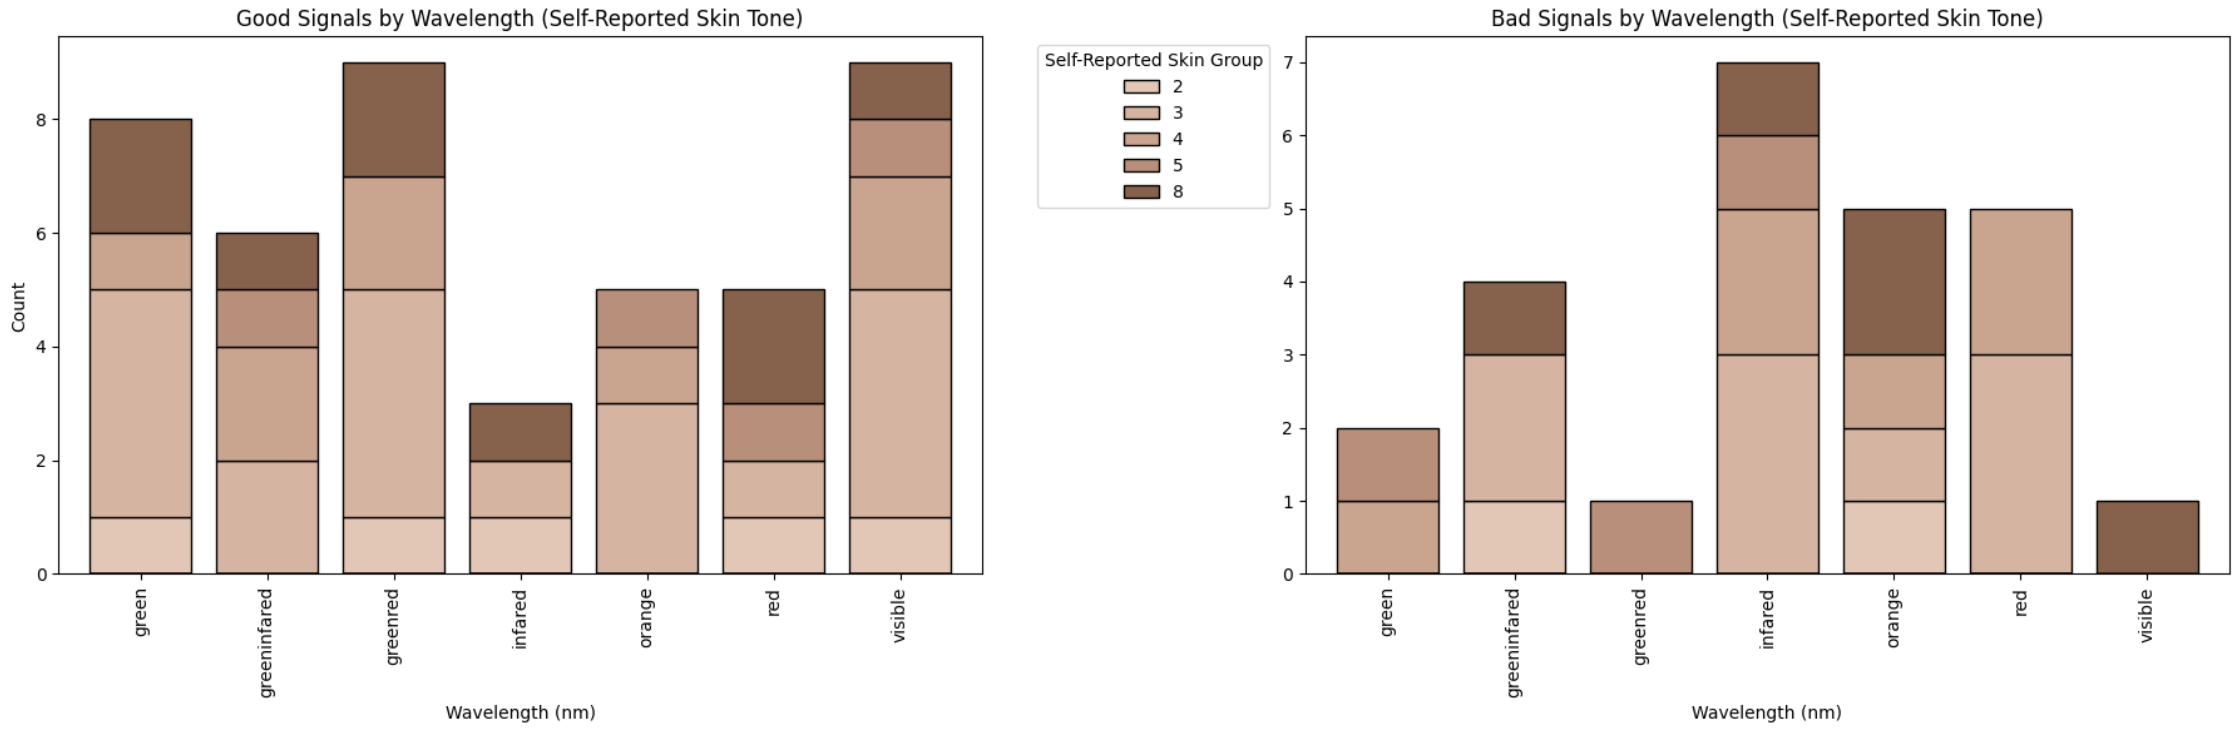
\includegraphics[width=\linewidth]{images/selfreport_hist.png}
    \caption{Signal Quality by Wavelength, stratified by skin tone using self report on the Fitzpatrick Scale.}
    \label{fig:selfreport_hist}
\end{figure}


\section{Discussion}

Our results suggest that the wavelength type used in photoplethysmography (PPG) significantly influences signal quality, while skin pigmentation shows minimal correlation with signal quality across various metrics. This finding contrasts with existing literature, which has often reported a noticeable impact of skin pigmentation on pulse oximetry accuracy and optical properties relevant to medical technologies \cite{al-halawani_review_2023}\cite{setchfield_effect_2024}. While this difference could be due to many factors, we want to stress the high variability exhibited by PPG devices, as also reported by Bent, et al. \cite{bent_investigating_2020}. 

The analysis clearly shows distinct variations in PPG quality among wavelength types. Specifically, wavelength combinations involving visible light—particularly the "Green and Red" and "Visible Light" combinations—yielded consistently higher quality signals compared to infrared wavelengths. The poor performance observed in infrared wavelengths primarily resulted from flatlined signals, indicating practical limitations in utilizing infrared alone for reliable PPG measurements at rest. This observation contrasts somewhat with previous literature that has broadly supported infrared for deep tissue penetration and low interference [4] [9]. However, our findings underscore the practical limitations and variability of infrared-based readings in certain contexts, possibly due to differences in environmental control, measurement setups, or the specific infrared wavelengths and sensor configurations used.

The minimal correlation between skin pigmentation and signal quality metrics suggests that, while skin pigmentation could theoretically affect optical properties, we did not establish a strong correlation in our findings under controlled environmental conditions. Our utilization of precise colorimetry tools like CIELab, as opposed to subjective scales, contributes robustness to our observations and addresses methodological gaps in previous research, where subjective assessments may have contributed to variability and inconclusive results [10][11].

Our study contributes to the ongoing conversation regarding the relationship between skin pigmentation and PPG signal quality by providing empirical data from controlled laboratory conditions and precise measurement methods. The insights derived here resonate with recent recommendations advocating for standardized and objective measurement approaches in skin pigmentation assessment [5].

\section{Conclusion}

One key limitation of our study was the relatively small sample size, which may have contributed to the high variability observed in the PPG quality scores. This variability likely influenced our inability to find statistically significant correlations between skin pigmentation and PPG signal quality metrics. Future research should incorporate a larger, more diverse participant sample to enhance statistical power and reliability of conclusions.

Additionally, while the CIELab measurement technique provided objective data on skin pigmentation, it has inherent limitations, such as sensitivity to lighting conditions and measurement angles. Incorporating more precise and specialized melonometry tools, as suggested by Vasudevan et al. \cite{vasudevan_melanometry_2024}, could improve the accuracy and consistency of skin pigmentation measurements in subsequent studies, thus potentially clarifying any existing relationships between skin pigmentation and PPG signal quality.

% To train this model, we utilized the open access Brno University of Technology Smartphone PPG Database (BUT PPG) \cite{nemcova_brno_2021}\cite{nemcova_brno_nodate} as the training set, which is comprised of 3,888 10-second 30 Hz recordings of PPGs from 50 subjects of 25 females and 25 males aged 19 to 76 years of age. The researchers measured PPG signals with smartphones while the participants were at rest and were prompted to perform other movements. Then signal quality was annotated by 3 to 5 annotators, where signal quality was considered good (with a binary label of 1) when two out of the three or three out of the five annotators provided a label of ‘good’ and signal quality was considered bad (with a binary label of 0) when the previous condition was not met. Because the signals in the BUT PPG dataset were recorded at a sampling rate of 30 Hz, we resampled the dataset to 50 Hz using Fourier-based interpolation. To normalize the data, we also scaled the raw values with min-max scaling. The model was evaluated on the accuracy, precision, recall, and F1 scores.

% Our collected data was then fed through the model to classify signal quality as a binary variable of either good (corresponding to label of 1) or bad (corresponding to label of 0). The proportion of good quality signals to poor quality signals were compared to the scores obtained from the SQI and SNR, in which higher scores correspond to better quality signals, as well as a quality score based on PSD, in which we calculated how much power lied in the 0.5 to 3 Hz range (the expected heart rate range) compared to total power. 

% \subsection{Potential Limitations}
% It may prove difficult to train a neural network on the BUT PPG dataset and use it for our PPG data collected using ExtHub, due to the systemic discrepancies that may arise from the methods of data collection; specifically, the difference in PPG hardware and the difference in testing environment. We attempt to reduce these discrepancies by normalizing both BUT and ExtHub PPG signals, as well as interpolating the BUT PPG signals up to 50 Hz, the same sampling frequency used by ExtHub. We hope to be able to achieve greater than 90\% accuracy on matching the ground truth label from the BUT dataset; however we realize that the task transfer may prove untenable for the model to overcome. We plan to account for this by assuming, unless proven otherwise, that the model will have similar prediction accuracy on the ExtHub data as it does on the BUT PPG dataset. 

\addtolength{\textheight}{-12cm}   % This command serves to balance the column lengths
                                  % on the last page of the document manually. It shortens
                                  % the textheight of the last page by a suitable amount.
                                  % This command does not take effect until the next page
                                  % so it should come on the page before the last. Make
                                  % sure that you do not shorten the textheight too much.

%%%%%%%%%%%%%%%%%%%%%%%%%%%%%%%%%%%%%%%%%%%%%%%%%%%%%%%%%%%%%%%%%%%%%%%%%%%%%%%%



%%%%%%%%%%%%%%%%%%%%%%%%%%%%%%%%%%%%%%%%%%%%%%%%%%%%%%%%%%%%%%%%%%%%%%%%%%%%%%%%



%%%%%%%%%%%%%%%%%%%%%%%%%%%%%%%%%%%%%%%%%%%%%%%%%%%%%%%%%%%%%%%%%%%%%%%%%%%%%%%%
% \section*{APPENDIX}


% \section*{ACKNOWLEDGMENT}



%%%%%%%%%%%%%%%%%%%%%%%%%%%%%%%%%%%%%%%%%%%%%%%%%%%%%%%%%%%%%%%%%%%%%%%%%%%%%%%%


\bibliographystyle{ieeetr}
\bibliography{citations}




\end{document}
